%! Author = angel
%! Date = 3/04/25

% Preamble
\documentclass[11pt]{article}

% Packages
\usepackage{amsmath,amssymb,amsthm}
\usepackage[letterpaper,margin=0.75in]{geometry}
\usepackage{pgfplots}
\usepackage{gensymb}
\usepackage{tikz}
\usepackage[usenames, dvipsnames]{xcolor}
\usepackage{fancyhdr}
\pgfplotsset{compat=1.18}
\usepackage{tikz-cd}

\usetikzlibrary{decorations.markings, arrows.meta}
% Document
\tikzset{
    marrow/.style={decoration={markings,mark=at position 0.5 with {\arrow{#1}}}, postaction=decorate}
}


\newcommand{\fahrenheit}{\degree \text{F}}

% Document
\begin{document}
    \noindent \textbf{Chapter 18: The First Law of Thermodynamics}
    \\ \noindent \newline Temperature measures the amount of energy of the particles of a given an object,
    which we feel as hot with more energy, and cold with less energy.
    We measure temperature in Kelvin (K),
    but also use the celsius scale (\celsius), and the fahrenheit scale (\fahrenheit):
    \begin{equation}
       T_C = T_K - 273.15\celsius \tag{Celsius}
    \end{equation}
    \begin{equation}
        T_F = \frac{9}{5}T_C + 32\celsius \tag{Fahrenheit}
    \end{equation}
    \noindent Temperature affects the phyiscal properties of an object, such as heat causing metal to expand.
    We can calculate the change in length over a change in temperature ($\celsius$ or K):
    \begin{equation}
        \Delta L = L \alpha \Delta T \tag{linear expansion}
    \end{equation}
    \noindent Where $\alpha$ and $ \beta = 3\alpha$ is the coefficient of linear expansion ($\celsius^{-1}$).
    For a change in volume we use:
    \begin{equation}
        \Delta V = V \beta \Delta T \tag{volume expansion}
    \end{equation}
    \noindent Now if we have an object in an environment, such as an iced soda can outside in the sun,
    its temperature rises quickly at first, but then the soda's temperature increasing rate slows down
    until it reaches the ambient temperature.
    We see that if the temperature of our system $T_s$ (the soda) and the environment $T_e$ are different, they
    will reach equilibrium.
    This change of temperature is the result of energy transfer called Heat Q (J).

            \begin{minipage}{0.3\textwidth} % Adjust width for graphs
                \hspace{-0.7cm}
                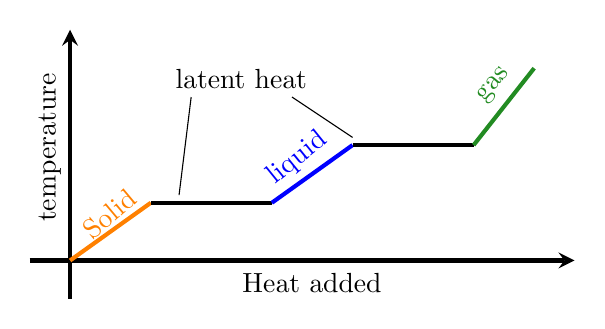
\begin{tikzpicture}
                    \tikzstyle{every path}=[line width=1.5pt]
                    \begin{axis}[
                        ytick=\empty,
                        xtick=\empty,
                        samples=1000,
                        axis lines=middle, % Draws both x and y axes at the middle
                        enlargelimits=false,
                        height=5cm,
                        width=8.5cm,
                        xmin=-2, xmax=25,
                        ymin=-2, ymax=12
                    ]
                        \draw[-,orange] (0,0) -- (4,3);
                        \draw[-,black] (4,3) -- (10,3);
                        \draw[-,blue] (10,3) -- (14,6);
                        \draw[-,black] (14,6) -- (20,6);
                        \draw[-,ForestGreen] (20,6) -- (23,10);
                        \draw[-,black,thin] (14,6.4) -- (11,8.5);
                        \draw[-,black,thin] (5.4,3.4) -- (6,8.5);
                        %\draw[orange, fill=orange] (4,3) circle (0.2) node[orange, above=0.2cm, left] {$S_1$};
                        \draw(3.5,3) node[orange, above=0.2cm, left, rotate=40] {Solid};
                        \draw(13,6) node[blue, above=0.2cm, left, rotate=39] {liquid};
                        \draw(22,9.5) node[ForestGreen, above=0.2cm, left, rotate=50] {gas};
                        \draw(12.3,8.6) node[black, above=0.2cm, left] {latent heat};
                        \draw(-1,9.5) node[black, above=0.2cm, left, rotate=90] {temperature};
                        \draw(16,-2) node[black, above=0.2cm, left] {Heat added};
                    \end{axis}
                \end{tikzpicture}
            \end{minipage}
            \hspace{1.6cm}
            \begin{minipage}[t]{0.56\textwidth}
                \vspace{-5em}
                \hspace{0.1cm}
                \\ \noindent When heat is added to system, the temperature of an object \emph{tends} to increase until
                an object reaches melting or vaporizing point where it will need more energy to change states.
                The latent heat L (cal/g or J/kg) of a material is the amount of energy required to change states:
                \begin{equation}
                     Q = mL \tag{latent heat}
                \end{equation}
            \end{minipage}

        \noindent \\ Where the \textcolor{orange}{\textbf{latent heat of fusion $L_f$}} is the transition between \textcolor{orange}{\textbf{solid and liquid}},
    while the \textcolor{ForestGreen}{\textbf{latent heat of vaporization $L_v$}} is the transition between \textcolor{ForestGreen}{\textbf{gas and liquid.}}
    Aside from heat, Calories and British thermal units (Btu) measure the amount of energy that would raise the temperature of 1g of water
    from $14.5\celsius$ to $15.5\celsius$ and 1 lb of water from $63\fahrenheit$ to $64\fahrenheit$ respectively.
    \begin{equation}
        1 \text{ cal} = 3.968 \times 10^{-3} \text{ Btu }= 4.1868 \text{ J} \notag
    \end{equation}

    \noindent With this, we can find the amount of heat used during a change of temperature,
    given the heat capacity C (J/K) of an object.
    \begin{equation}
        Q = C \Delta T = C(T_f - T_i) \tag{heat capacity}
    \end{equation}
    However, the heat capacity is different for every system, depending on the material of an object, and its mass.
    The heat capacity is the product of the heat specific heat c ($\frac{J}{kg \cdot K}$) and its mass.
    With this, the specific heat unit conversions are now:
     \begin{equation}
          1 \text{ cal/g} = 3.968 \times 10^{-3} \text{ Btu/lb }= 4.1868 \text{ J/(K $\times$ kg)} \notag
    \end{equation}
    \noindent Now we can find heat used over a change of temperature given the specific heat constant and mass:
    \begin{equation}
        Q = cm \Delta T = cm(T_f - T_i) \tag{specific heat}
    \end{equation}
    \noindent Remembering that heat is energy, we can use Power ($W = \frac{J}{s}$) and time:
    \begin{equation}
        Q = Pt \tag{power}
    \end{equation}

    \newpage
    \noindent \textbf{Chapter 18: The First Law of Thermodynamics}
    \\ \noindent \newline As energy can neither be created nor destroyed, the first Law of Thermodynamics states:
    \begin{equation}
        \Delta E_{int} = E_f - E_i = Q - W \tag{first law}
    \end{equation}
    \noindent And if the system undergoes differential change:
    \begin{equation}
        dE = dQ - dW \tag{first law}
    \end{equation}
    The principle of energy conservation shows that the change of our internal energy in the system ($\Delta E_{int}$)
    is found by heat added to system Q while removing the work done by the system.
    Imagine you are charging your phone, causing energy to transfer to the phone;
    this is work done on your phone (system).
    Now if your phone was playing a movie, it expends energy, causing work by your phone (system).
    With this in mind, we can start working with how gas can exchange energy with its surroundings through work:
    \begin{equation}
        W = \int dW = \int_{v_i}^{v_f} p \text{ } dV \tag{work}
    \end{equation}
    In a system such as an engine, a piston will compress gas in the engine, doing work on the system by
    causing a change in volume.
    Since work is a force done over a displacement, $dW = F \cdot dx$,
    we can rewrite the force in terms of area and pressure $F = pA$.
    This gives us $dW = pA \cdot dx = p \text{ }dV$

    \begin{minipage}{0.3\textwidth} % Adjust width for graphs
        \hspace{-0.7cm}
        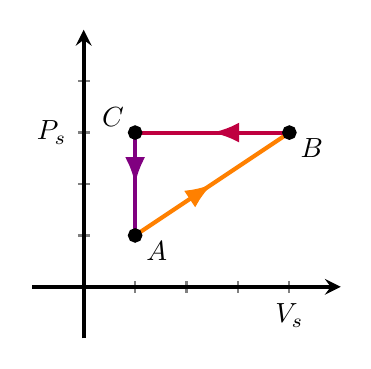
\begin{tikzpicture}
            \tikzstyle{every path}=[line width=1.5pt]
            \begin{axis}[
                ytick=\empty,
                xtick=\empty,
                samples=1000,
                axis lines=middle, % Draws both x and y axes at the middle
                enlargelimits=false,
                height=5.5cm,
                width=5.5cm,
                xmin=-1, xmax=5,
                ymin=-1, ymax=5,
                tick style=thick,
                xtick={1,2,3,4},
                ytick={1 , 2, 3, 4},
                xticklabels={,,,$V_s$},
                yticklabels={,, $P_s$}
            ]
                \draw[-,orange,marrow=Latex] (1,1) -- (4,3);
                \draw[-,purple,marrow=Latex] (4,3) -- (1,3);
                \draw[-,violet,marrow=Latex] (1,3) -- (1,1);
                \draw[fill=black] (1,1) circle (0.1) node[below=0.2cm, right] {$A$};
            \draw[fill=black] (4,3) circle (0.1) node[below=0.2cm, right] {$B$};
            \draw[fill=black] (1,3) circle (0.1) node[above=0.2cm, left] {$C$};
            \end{axis}
        \end{tikzpicture}
    \end{minipage}
    \hspace{-1.5cm}
    \begin{minipage}[t]{0.75\textwidth}
        \vspace{-5em}
        \hspace{0.5cm}
        \\ \noindent Here we have a graph of a $p-V$ diagram where a gas undergoes compression and expansion.
        Let $P_s = 30 \text{ N}/m^2$ and $V_s = 4.0m^3$.
        To find the net energy added to the system, we need to find how much work was done for each
        segment, $W_{AB}, W_{BC}$ and $W_{CA}$. Lets start with $W_{BC}$, since pressure $p$ is constant through the path:
        \begin{equation}
           W_{BC} = \int_{V_s}^{\frac{1}{4}V_s} p \text{ } dV = P_sW\Big|_{V_s}^{\frac{1}{4} V_s} = P_s [\frac{1}{4}V_s - V_s]
           = P_s[-\frac{3}{4}V_s] = -90J\notag
        \end{equation}
    \end{minipage}

    \vspace{2em}
\noindent We see that the system did 90J of work. Now let's take a look at $W_{CA}$.
    Note that the volume does not change, so the integral's bounds will result in 0,
    giving $W_{CA} = 0$. Lastly, to find $W_{AB}$ we will need to treat pressure as a
    function of volume. In this case we have two points $A$ and $B$,
    so we will use the line formula to give us this integral:
    \begin{equation}
        W_{AB} = \int_{\frac{1}{4}V_s}^{V_s} \frac{10}{3} + \frac{20}{3}V dV
        = 60 J \notag
    \end{equation}
    Now the net work $W_{net} = W_{AB} + W_{BC} + W_{CA}$ which gives us $-30J.$
    Given that $\Delta E_{int} = - W = 30J$,
    this means that 30J of energy was done on the system, increasing its heat.
    In this case, we did not consider the transfer of heat between the environment and the system,
    resulting in $Q = 0$, know as an adiabatic process.
    In fact 4 special cases for the first law of Thermodynamics:
    \begin{equation}
        \Delta E_{int} = -W \tag{adiabatic process}
    \end{equation}
    When no transfer of heat between the environment and the system.
    \begin{equation}
       \hspace{4cm} \Delta E_{int} = Q\tag{Constant-volume process}
    \end{equation}
    When the volume of a system is constant resulting in $W = 0$.
    \begin{equation}
        \Delta Q = W\tag{Cyclical process}
    \end{equation}
    After a process has occurred, returning to its original state,
    resulting in the system's internal energy.
    \begin{equation}
        \Delta E_{int} = 0 \tag{Free expansions}
    \end{equation}

    \newpage
    \noindent \textbf{Chapter 18: The First Law of Thermodynamics}
    \\ \noindent \newline If we leave the iced soda can outside,
    the energy is transferred from the outside environment to the inside
    through \textbf{conduction} (W):
    \begin{equation}
        P_{cond} = \frac{Q}{t} = kA\cdot \frac{\Delta T}{L} \tag{conduction}
    \end{equation}
    \noindent Where $k$ is the conductivity of your material,
    $A$ is the area of the barrier, and $L$ is the length.
    As with conduction we can also measure the resistance,
    or how good a material at a specific length is at insulating heat:
    \begin{equation}
        R = \frac{L}{K} \tag{resistance}
    \end{equation}
    \noindent Sometimes there will be multiple layers of a different materials
    between hot and cold areas. We can use the resistance of each material
    to measure the whole energy transfer rate:
    \begin{equation}
        P_{cond} = \frac{A \Delta T}{\Sigma \frac{L}{K} } \tag{conduction}
    \end{equation}
    \noindent If we have a candle in a cold environment,
    we can feel the heat radiating out of the candle.
    This energy transfer is \textbf{thermal radiation}
    which is when energy is exchanged through electromagnetic waves.
    The rate at the energy is emitted by the system is given by:
    \begin{equation}
        P_{rad} = \alpha \epsilon A T_{obj}^4 \tag{radiation rate}
    \end{equation}
    \noindent Here, the temperature of the object is in Kelvin,
    $\alpha = 5.6704 \times 10^8 W/m^2\cdot K^4$ is the Stefan–Boltzmann constant
    and $\epsilon$ is the emissivity of the object’s surface.
    However, an object can also absorb thermal radiation:
    \begin{equation}
        P_{abs} = \alpha \epsilon A T_{env}^4 \tag{absorption rate}
    \end{equation}
    With this we can find the net power transfer where a positive value
    signifies energy is absorbed while a negative value shows that energy is lost:
    \begin{equation}
        P_{net} = P_{abs} - P_{rad} = \alpha \epsilon A (T_{env}^4 - T_{obj}^4) \tag{net power}
    \end{equation}
    


\end{document}